\documentclass[a4paper, 12pt] {article}

\usepackage[margin=1in]{geometry}
\usepackage[framemethod=TikZ]{mdframed}
\usepackage{graphicx}
\usepackage{xcolor,colortbl}
\usepackage{listings} % Allows code-listings
\usepackage{wrapfig}
\usepackage{courier} % proper monospace font for code
\usepackage{lscape}
\usepackage[utf8]{inputenc}
\usepackage[norsk]{babel}
\usepackage[T1]{fontenc}
\usepackage{rotating}
\usepackage{epstopdf}
\usepackage{hyperref} %linking fra content  table
\usepackage{xstring} %string-manipulation
\usepackage{enumitem} %used for enumerate-manipulation
\usepackage{float} %used to properly place float-objects (figures)
\usepackage{titlesec, blindtext, color}
\usepackage{tabularx,ragged2e,booktabs,caption}
\usepackage{ulem} %used for strikeout
\usepackage{verbatim} %used for block-commenting
\usepackage[toc,page]{appendix}
\usepackage{url}
\usepackage{amsmath}
\usepackage{tikz}
\usetikzlibrary{shapes}

\definecolor{gray75}{gray}{0.75}
\definecolor{gray1}{gray}{0.97}
\definecolor{gray2}{gray}{0.90}
\definecolor{gray3}{gray}{0.80}
\definecolor{gray4}{gray}{0.63}

\lstset{
    basicstyle=\footnotesize\ttfamily, % Standardschrift
    %numbers=left,               % Ort der Zeilennummern
    numberstyle=\tiny,          % Stil der Zeilennummern
    %stepnumber=2,               % Abstand zwischen den Zeilennummern
    numbersep=5pt,              % Abstand der Nummern zum Text
    tabsize=2,                  % Groesse von Tabs
    extendedchars=\true,         %
    breaklines=true,            % Zeilen werden Umgebrochen
    keywordstyle=\color{red},
    frame=b,         
 %  keywordstyle=[1]\textbf,    % Stil der Keywords
 %  keywordstyle=[2]\textbf,    %
 %  keywordstyle=[3]\textbf,    %
 %  keywordstyle=[4]\textbf,   \sqrt{\sqrt{}} %
    % stringstyle=\color{white}\ttfamily, % Farbe der String
    showspaces=false,           % Leerzeichen anzeigen ?
    showtabs=false,       % Tabs anzeigen ?
    inputencoding=utf8,
    xleftmargin=17pt,
    framexleftmargin=17pt,
    framexrightmargin=5pt,
    framexbottommargin=4pt,
    %backgroundcolor=\color{lightgray},
    showstringspaces=false      % Leerzeichen in Strings anzeigen ? 
}


%\DeclareCaptionFont{blue}{\color{blue}} 

%\captionsetup[lstlisting]{singlelinecheck=false, labelfont={blue}, textfont={blue}}
\usepackage{caption}
\DeclareCaptionFont{white}{\color{white}}
\DeclareCaptionFormat{listing}{\colorbox[cmyk]{0.43, 0.35, 0.35,0.01}{\parbox{\textwidth}{\hspace{15pt}#1#2#3}}}
\captionsetup[lstlisting]{format=listing,labelfont=white,textfont=white, singlelinecheck=false, margin=0pt, font={bf,footnotesize}}


\newcommand{\hsp}{\hspace{20pt}}
\newcommand{\HRule}{\rule{\linewidth}{0.5mm}}



\newcommand{\img}[2]{ %images with borders
	\begin{figure}[H]
	\centering
	\fcolorbox{black}{black}{\includegraphics[width=14cm]{img/#1}}
	\caption[#2]{#2}
	\end{figure}
}

\newcommand{\imgC}[3]{ %images with borders and custom parameters
	\begin{figure}[H]
	\centering
	\fcolorbox{black}{black}{\includegraphics[#2]{img/#1}}
	\caption[#3]{#3}
	\end{figure}
}


\newcommand{\liste}[1]{\begin{enumerate}[label=\textbf{#1:\arabic*}]}
\newcommand{\inn}{\begin{enumerate}[label*=\textbf{.\arabic*}]}
\newcommand{\ut}{\end{enumerate}}


\newcommand{\refer}[5]{\bibitem {#1} #2. "#3" \textit{#4} (#5).}

%\newcommand{\labs}{\label{sec:utdypning}}
%\newcommand{\labl}[1]{\label{itm:#1}}
%\newcommand{\refs}{(se side~\pageref{sec:utdypning})}
%\newcommand{\refl}[1]{\ref{itm:#1} - }


%\parindent=5pt
%\baselineskip=0pt
%\parskip=0pt

\hypersetup{ %Brukes for � fjerne farger fra linker i content table
    colorlinks,
    citecolor=black,
    filecolor=black,
    linkcolor=black,
    urlcolor=black
}

\titleformat{\chapter}[hang]{\Huge\bfseries}{\thechapter\hsp\textcolor{gray75}{|}\hsp}{0pt}{\Huge\bfseries}




\begin{document}
\pagenumbering{Roman}
% Upper part of the page. The '~' is needed because \\
% only works if a paragraph has started.
\begin{titlepage}
\begin{center}

\includegraphics[width=0.15\textwidth]{img/ntnulogo.PNG}~\\[1cm]

\textsc{\LARGE NTNU}\\[1.5cm]

\textsc{\Large TDT4145 - Datamodellering og databasesystemer}\\[0.5cm]

% Title
\HRule \\[0.4cm]
{ \huge \bfseries Øving 3}\\[0.5cm]
{\large \textit{Mathias Ose og \O yvind Robertsen}}\\[0.2cm]
\HRule \\[1.5cm]



\vfill

% Bottom of the page
{\large \today}
\end{center}
\end{titlepage}

\newpage

\tableofcontents
\newpage

\pagenumbering{arabic}

\section{Oppgave 1}

\subsection{Deloppgave 1}
\begin{figure}[h!]
    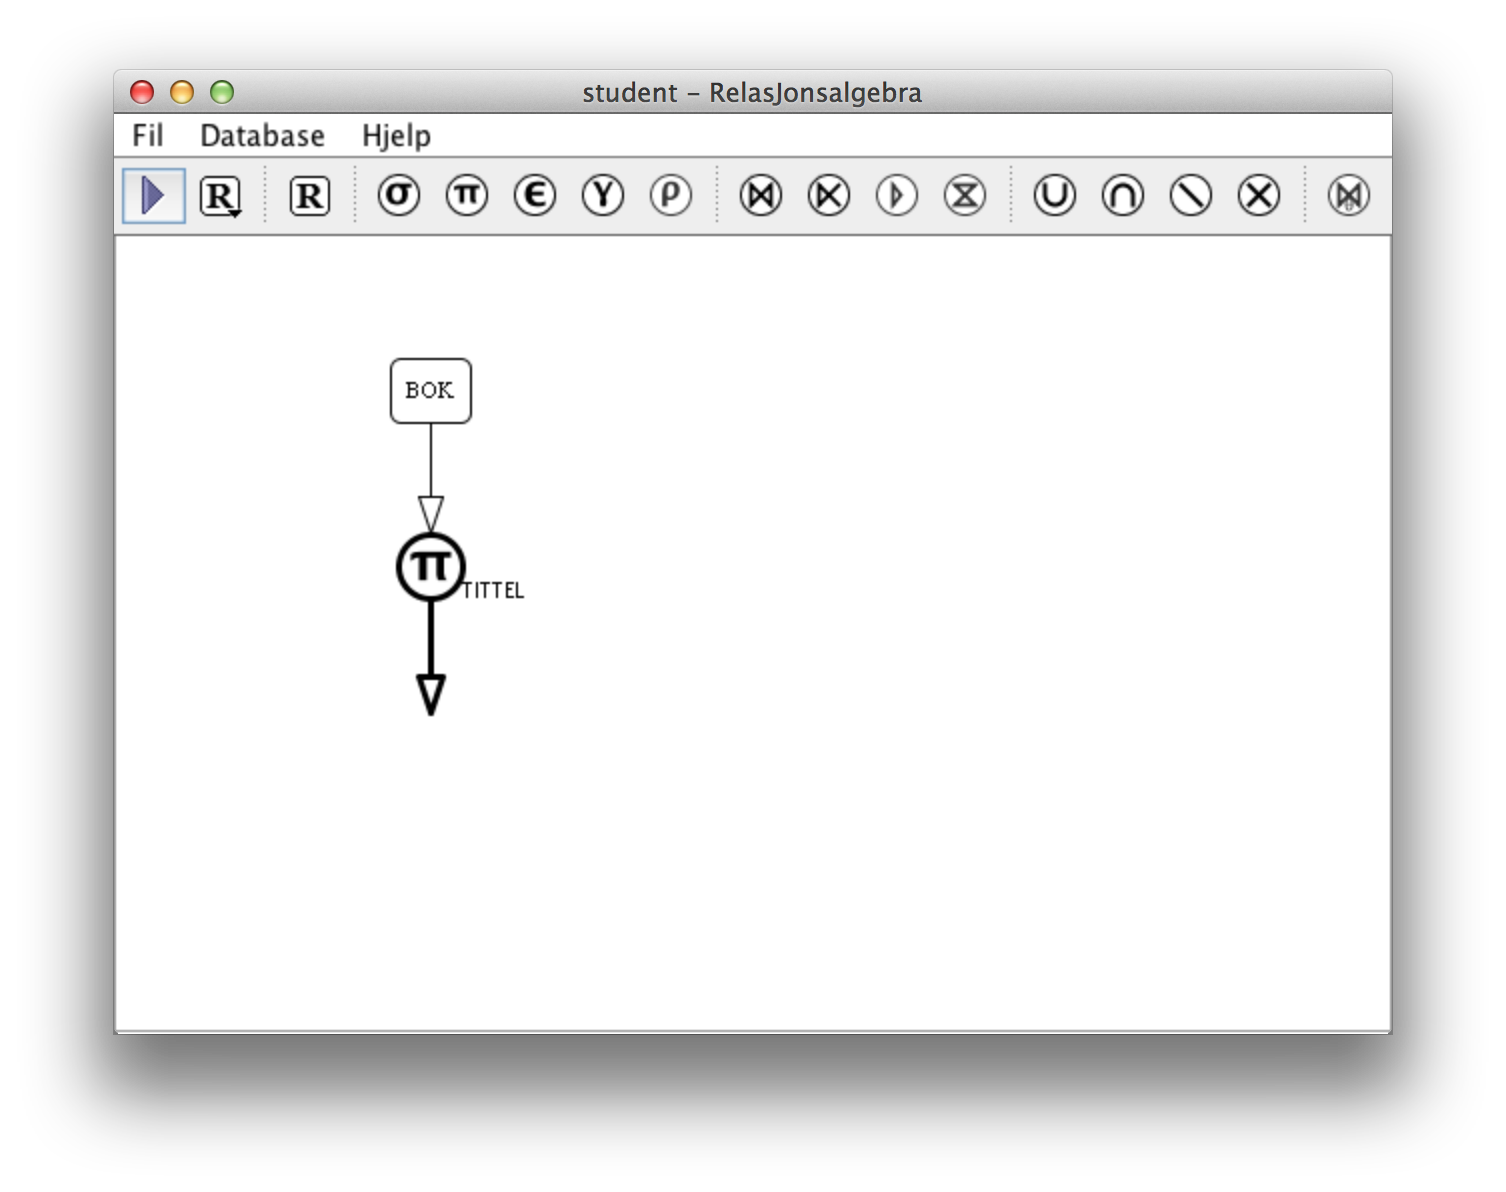
\includegraphics[width=\linewidth]{img/1-1.png}
    \caption{Spørring for oppg. 1.1 \label{img:1.1}}
\end{figure}
\newpage

\subsection{Deloppgave 2}
\begin{figure}[h!]
    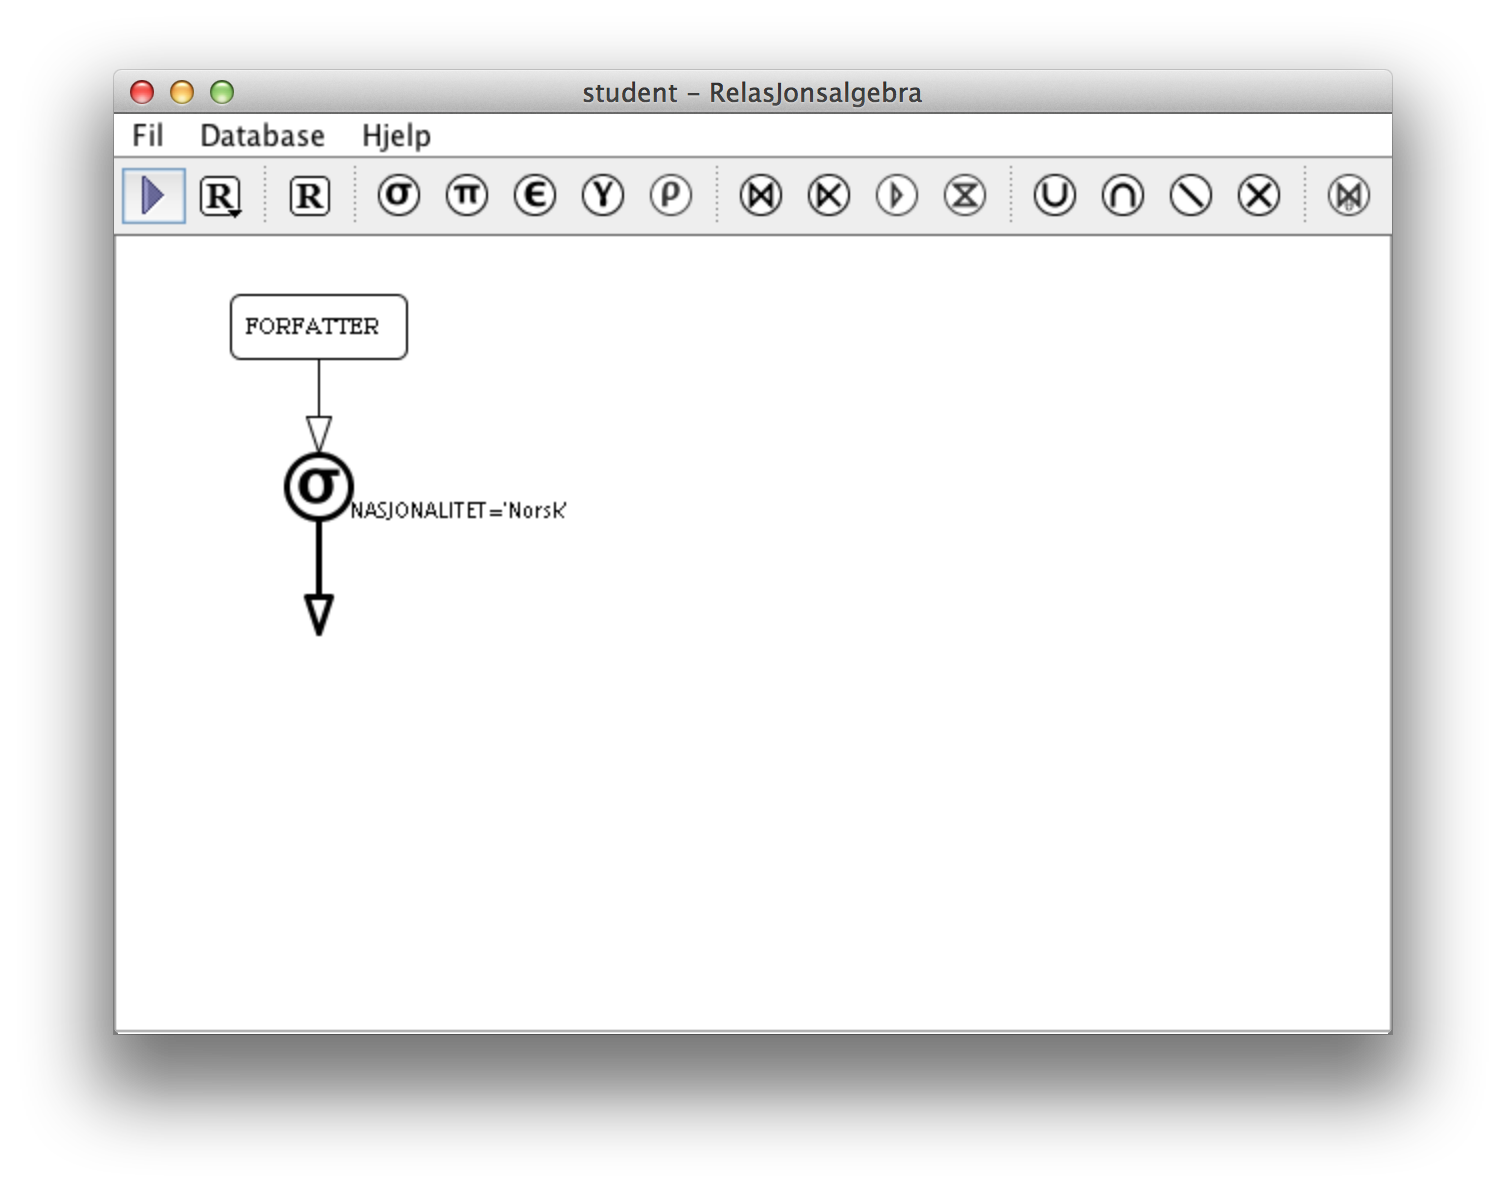
\includegraphics[width=\linewidth]{img/1-2.png}
    \caption{Spørring for oppg. 1.2 \label{img:1.2}}
\end{figure}
\newpage

\subsection{Deloppgave 3}
\begin{figure}[h!]
    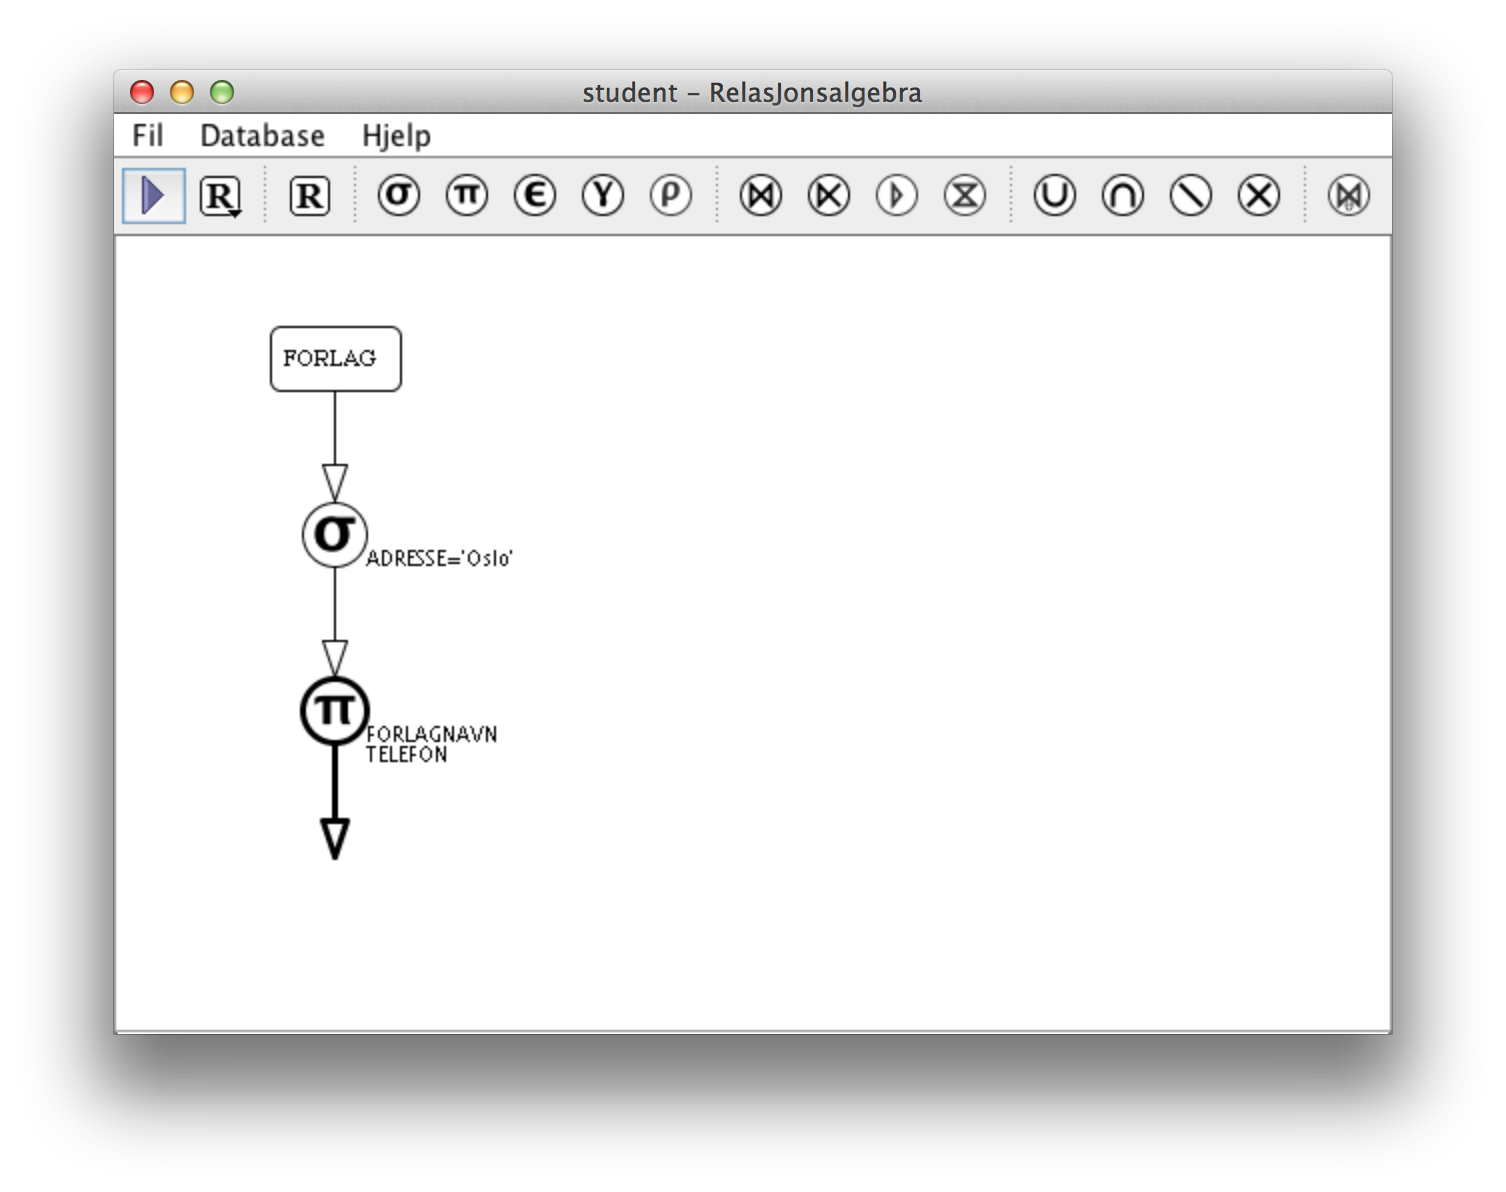
\includegraphics[width=\linewidth]{img/1-3.png}
    \caption{Spørring for oppg. 1.3 \label{img:1.3}}
\end{figure}
\newpage

\subsection{Deloppgave 4}
\begin{figure}[h!]
    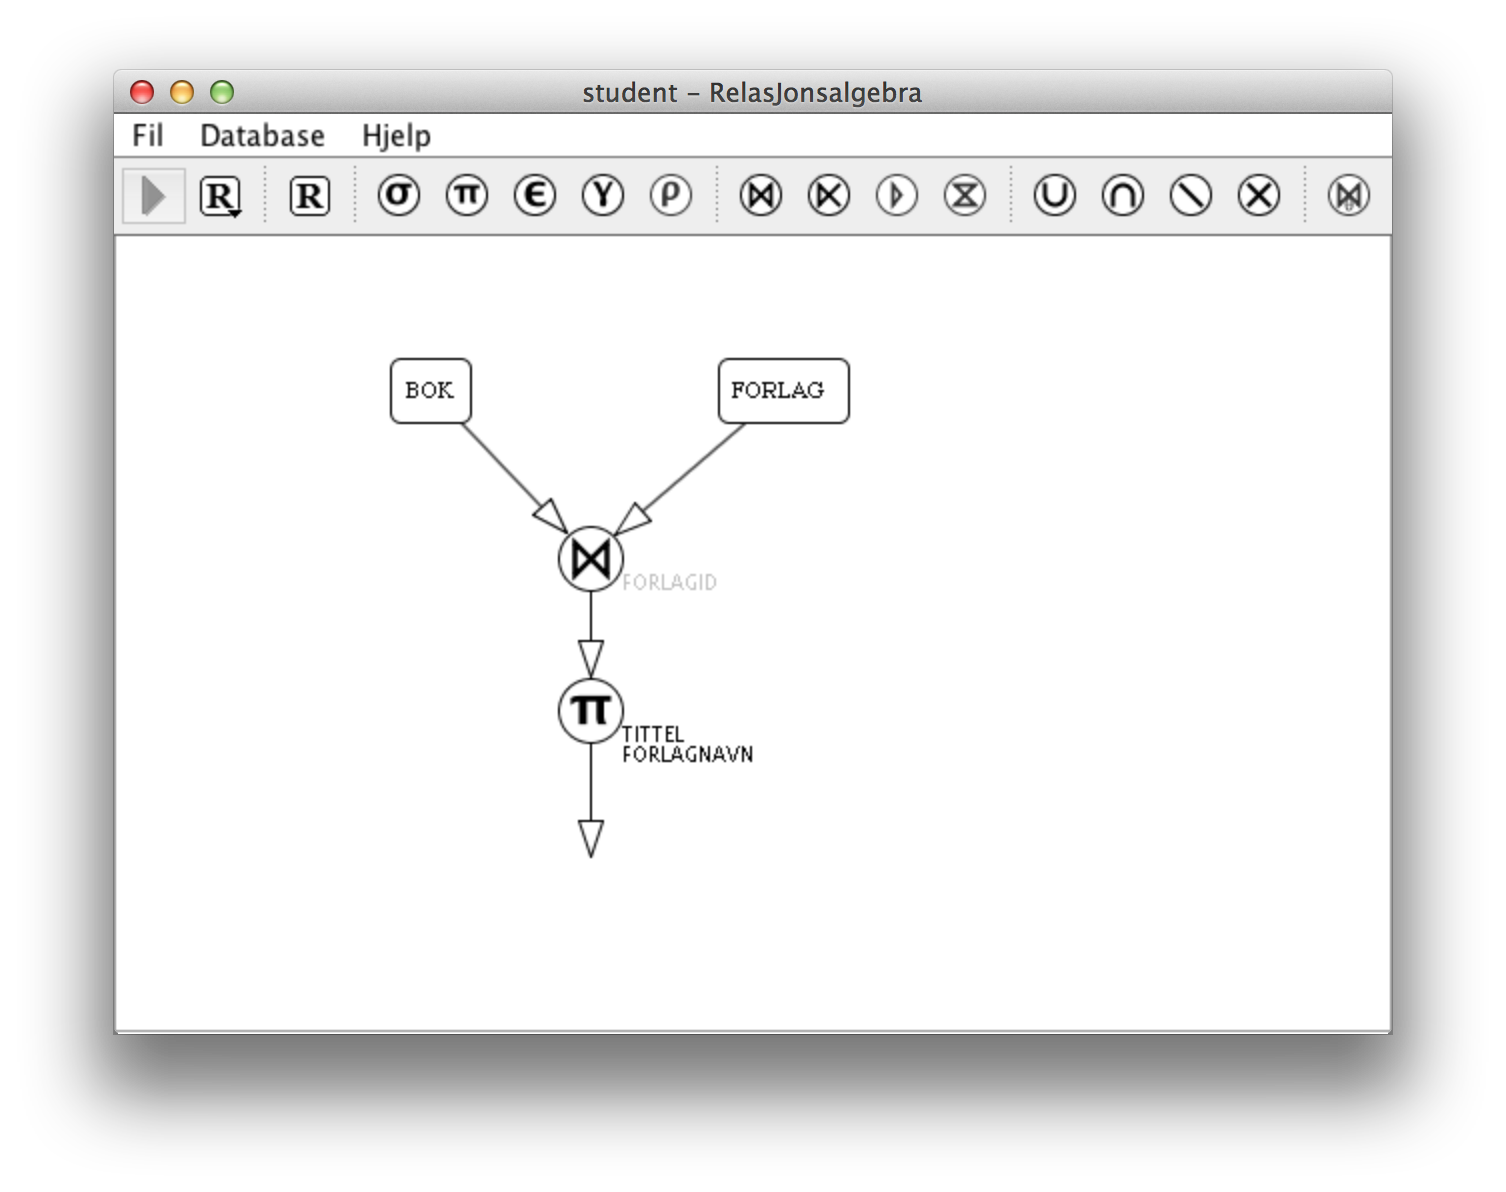
\includegraphics[width=\linewidth]{img/1-4.png}
    \caption{Spørring for oppg. 1.4 \label{img:1.4}}
\end{figure}
\newpage

\subsection{Deloppgave 5}
\begin{figure}[h!]
    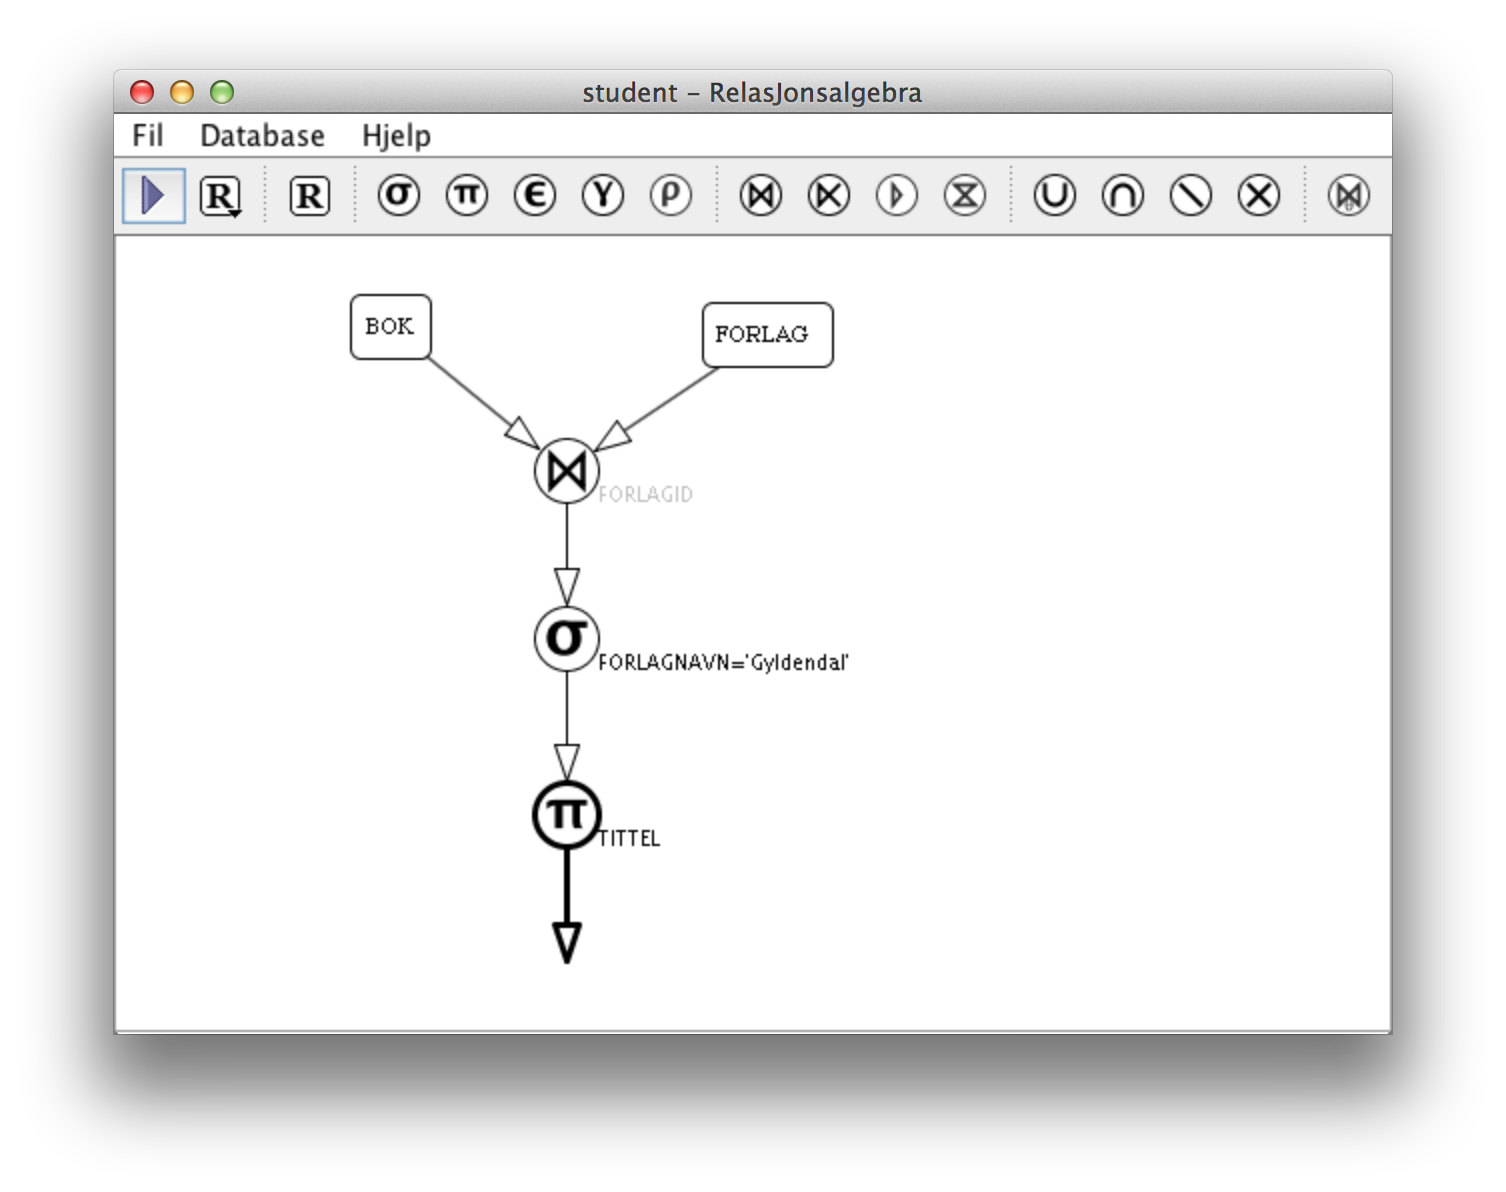
\includegraphics[width=\linewidth]{img/1-5.png}
    \caption{Spørring for oppg. 1.5 \label{img:1.5}}
\end{figure}
\newpage

\subsection{Deloppgave 6}
\begin{figure}[h!]
    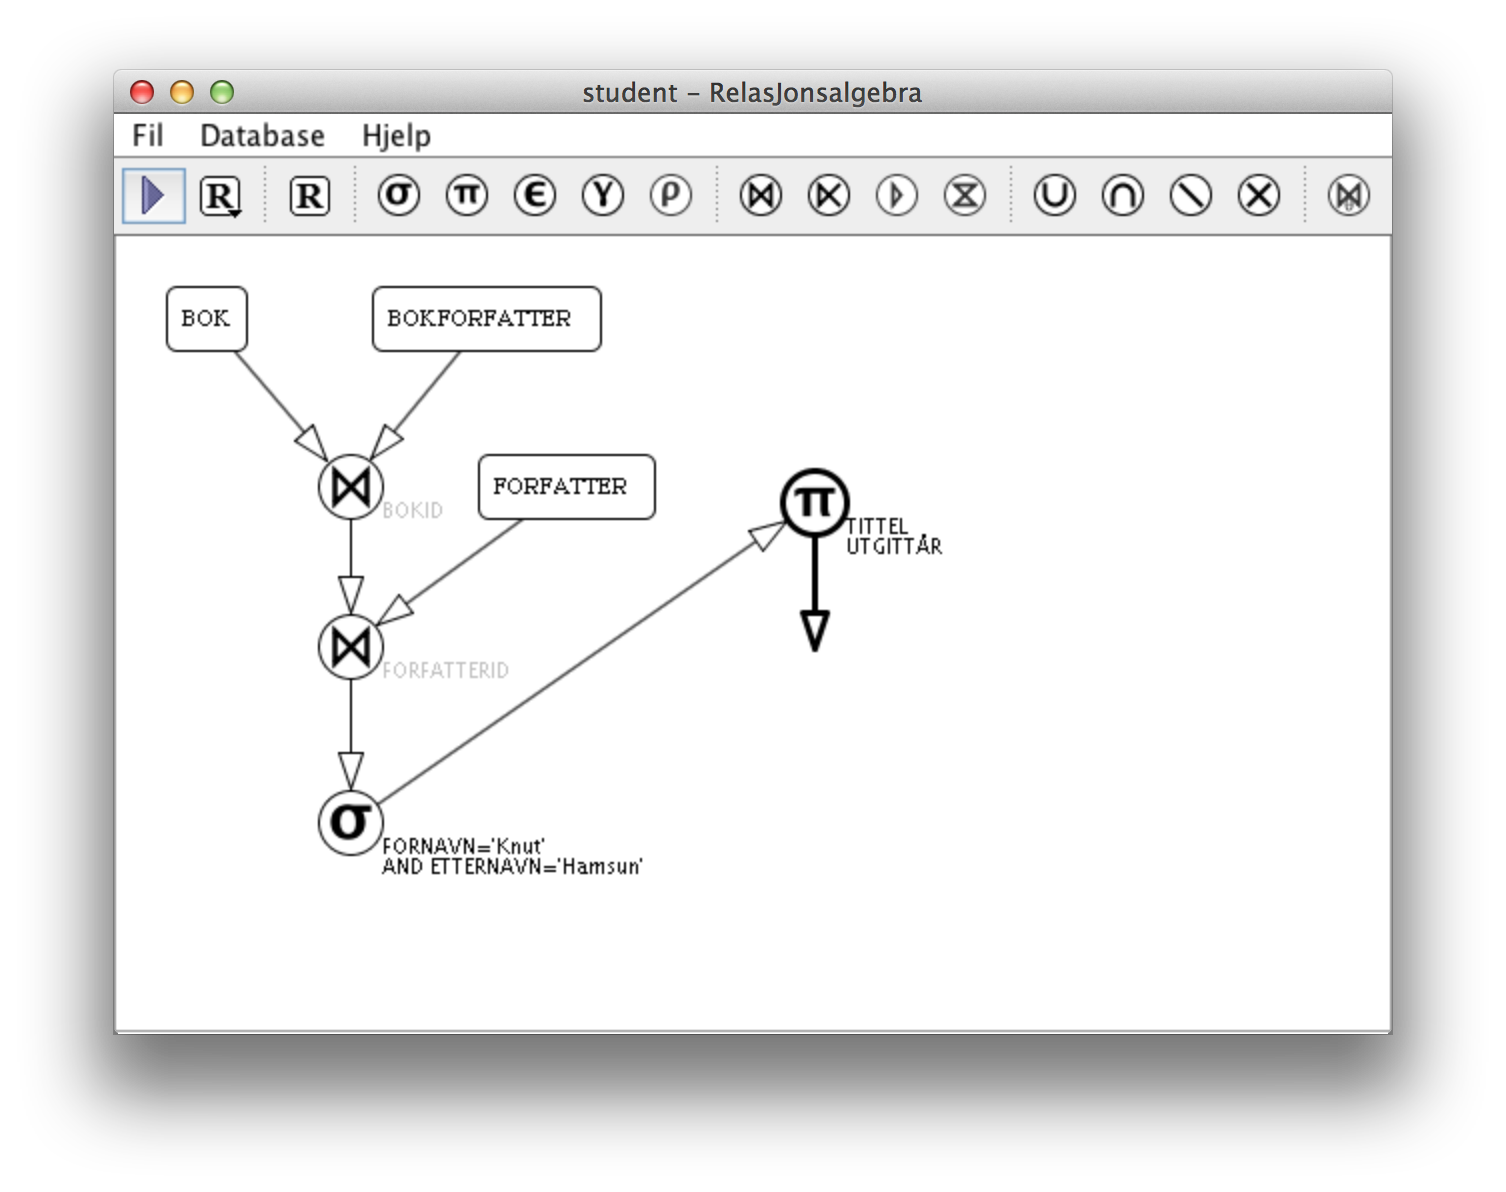
\includegraphics[width=\linewidth]{img/1-6.png}
    \caption{Spørring for oppg. 1.6 \label{img:1.6}}
\end{figure}
\newpage

\subsection{Deloppgave 7}
\begin{figure}[h!]
    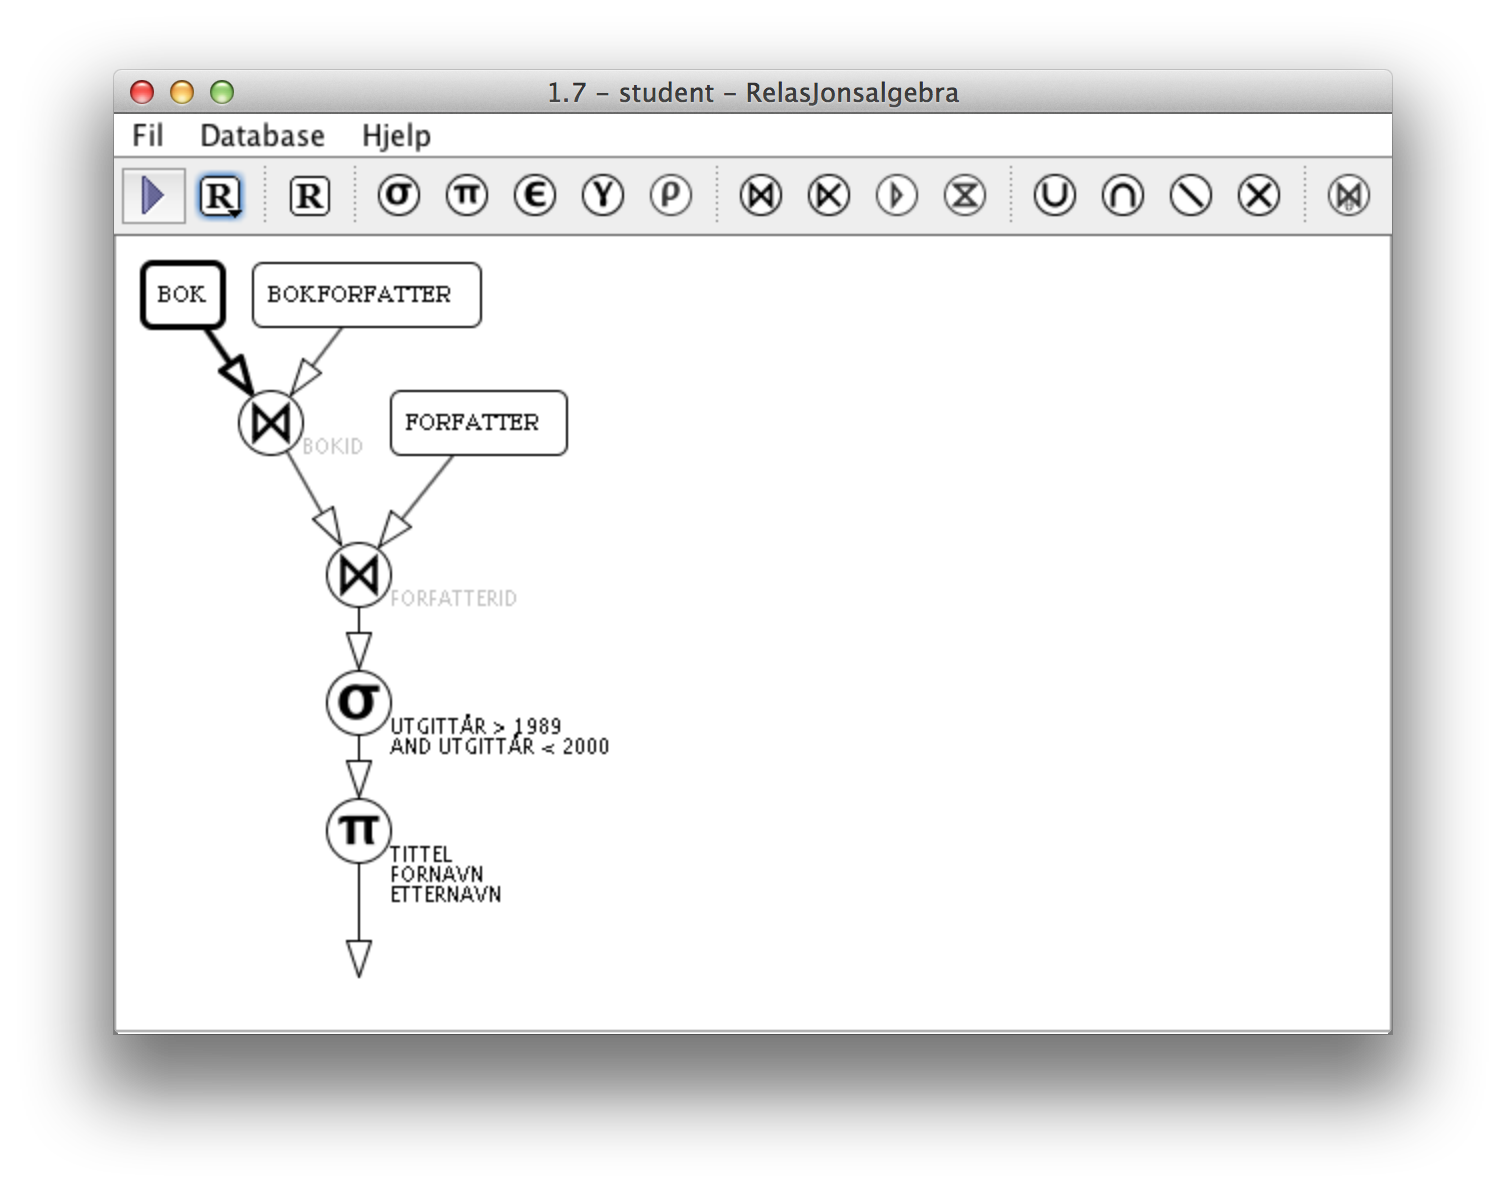
\includegraphics[width=\linewidth]{img/1-7.png}
    \caption{Spørring for oppg. 1.7 \label{img:1.7}}
\end{figure}
\newpage

\subsection{Deloppgave 8}
\begin{figure}[h!]
    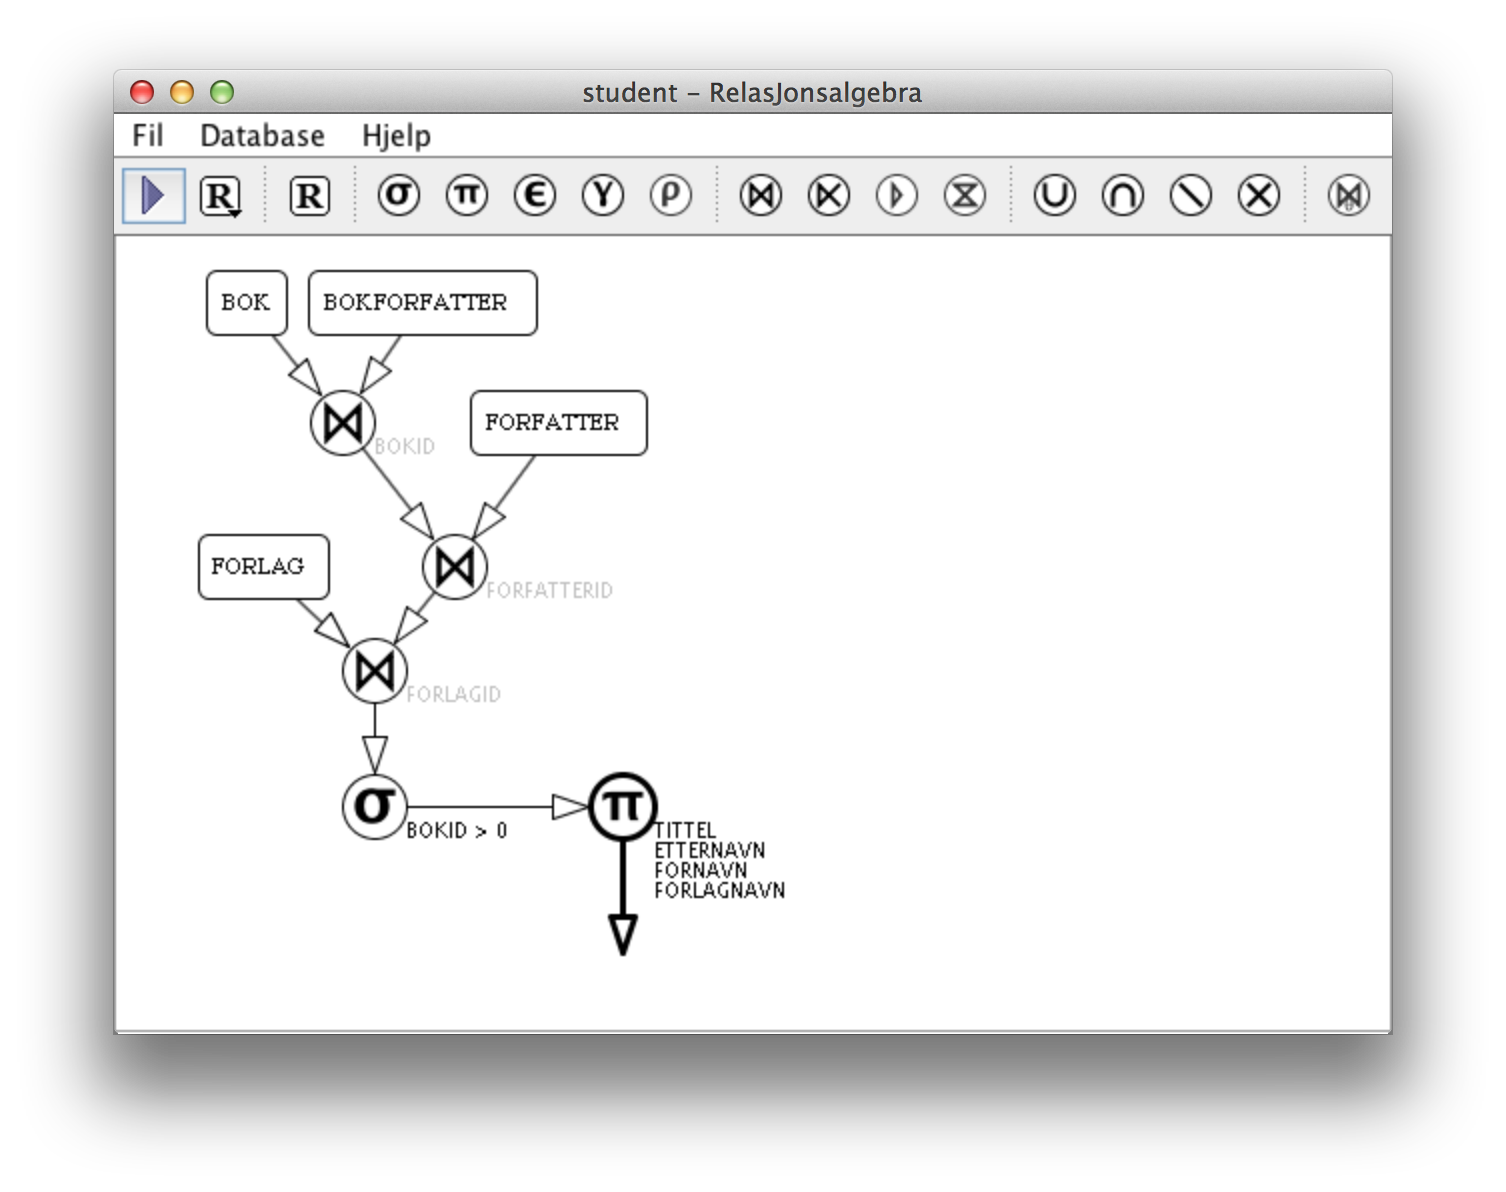
\includegraphics[width=\linewidth]{img/1-8.png}
    \caption{Spørring for oppg. 1.8 \label{img:1.8}}
\end{figure}
\newpage

\subsection{Deloppgave 9}
\begin{figure}[h!]
    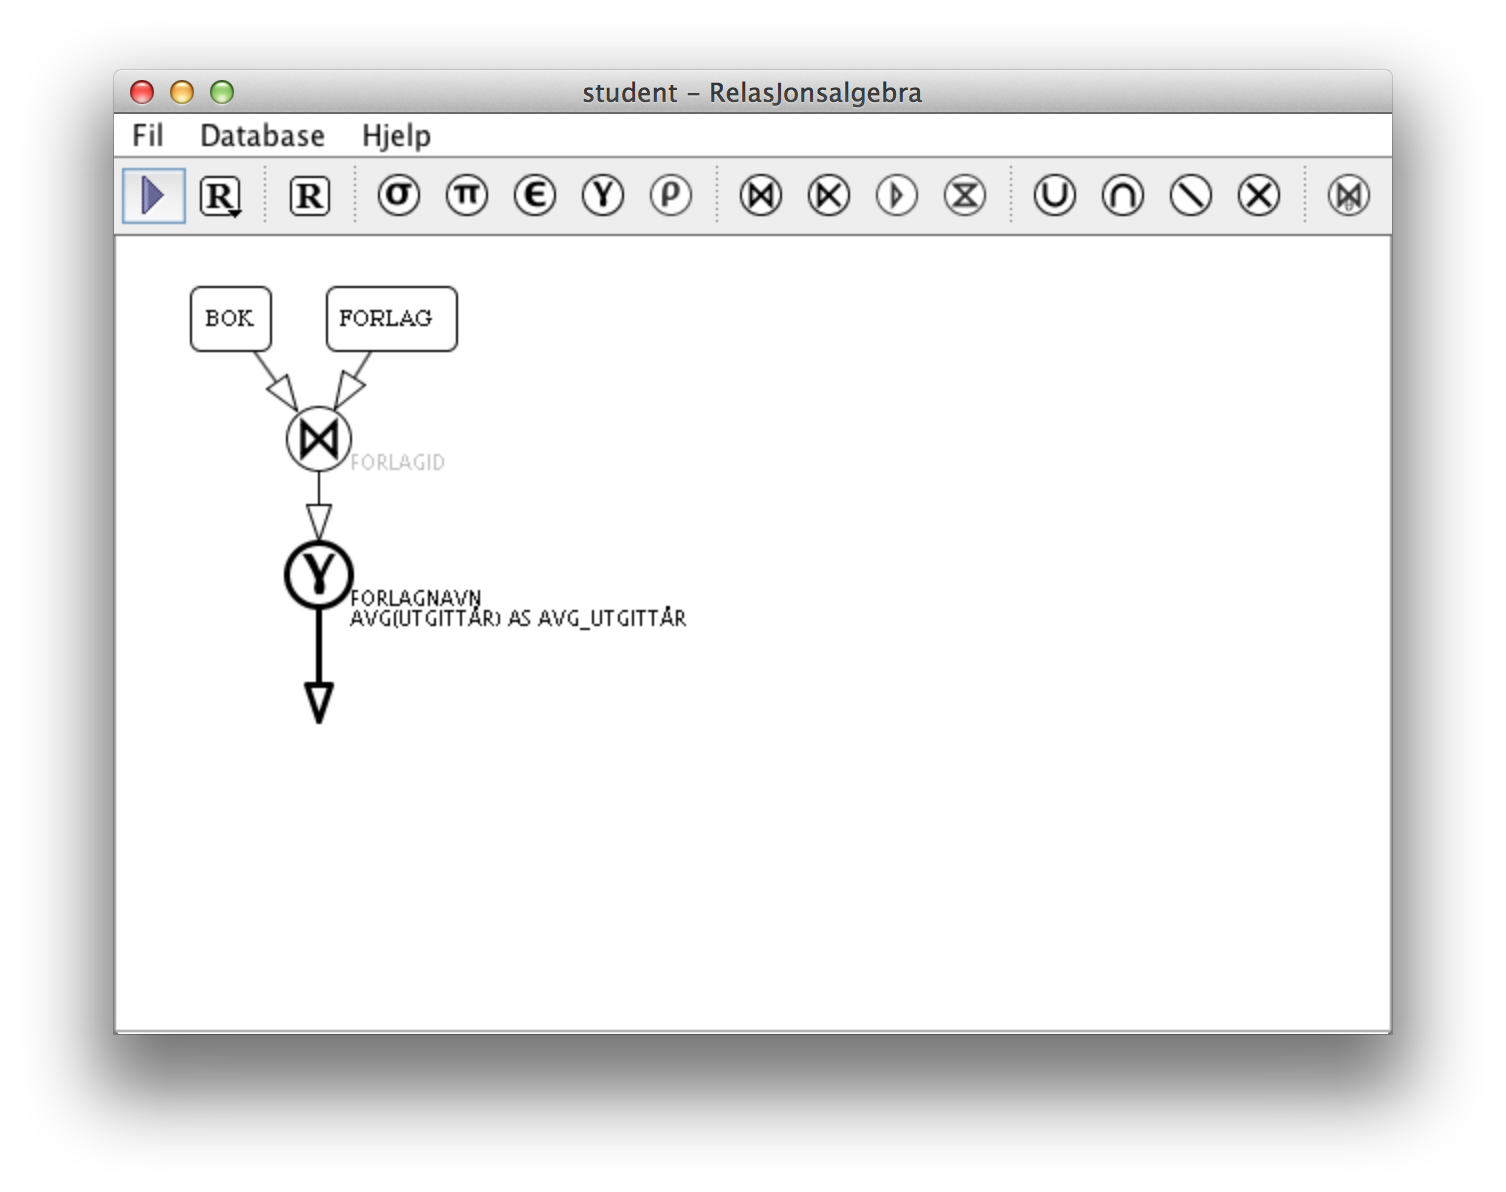
\includegraphics[width=\linewidth]{img/1-9.png}
    \caption{Spørring for oppg. 1.9 \label{img:1.9}}
\end{figure}
\newpage

\subsection{Deloppgave 10}
\begin{figure}[h!]
    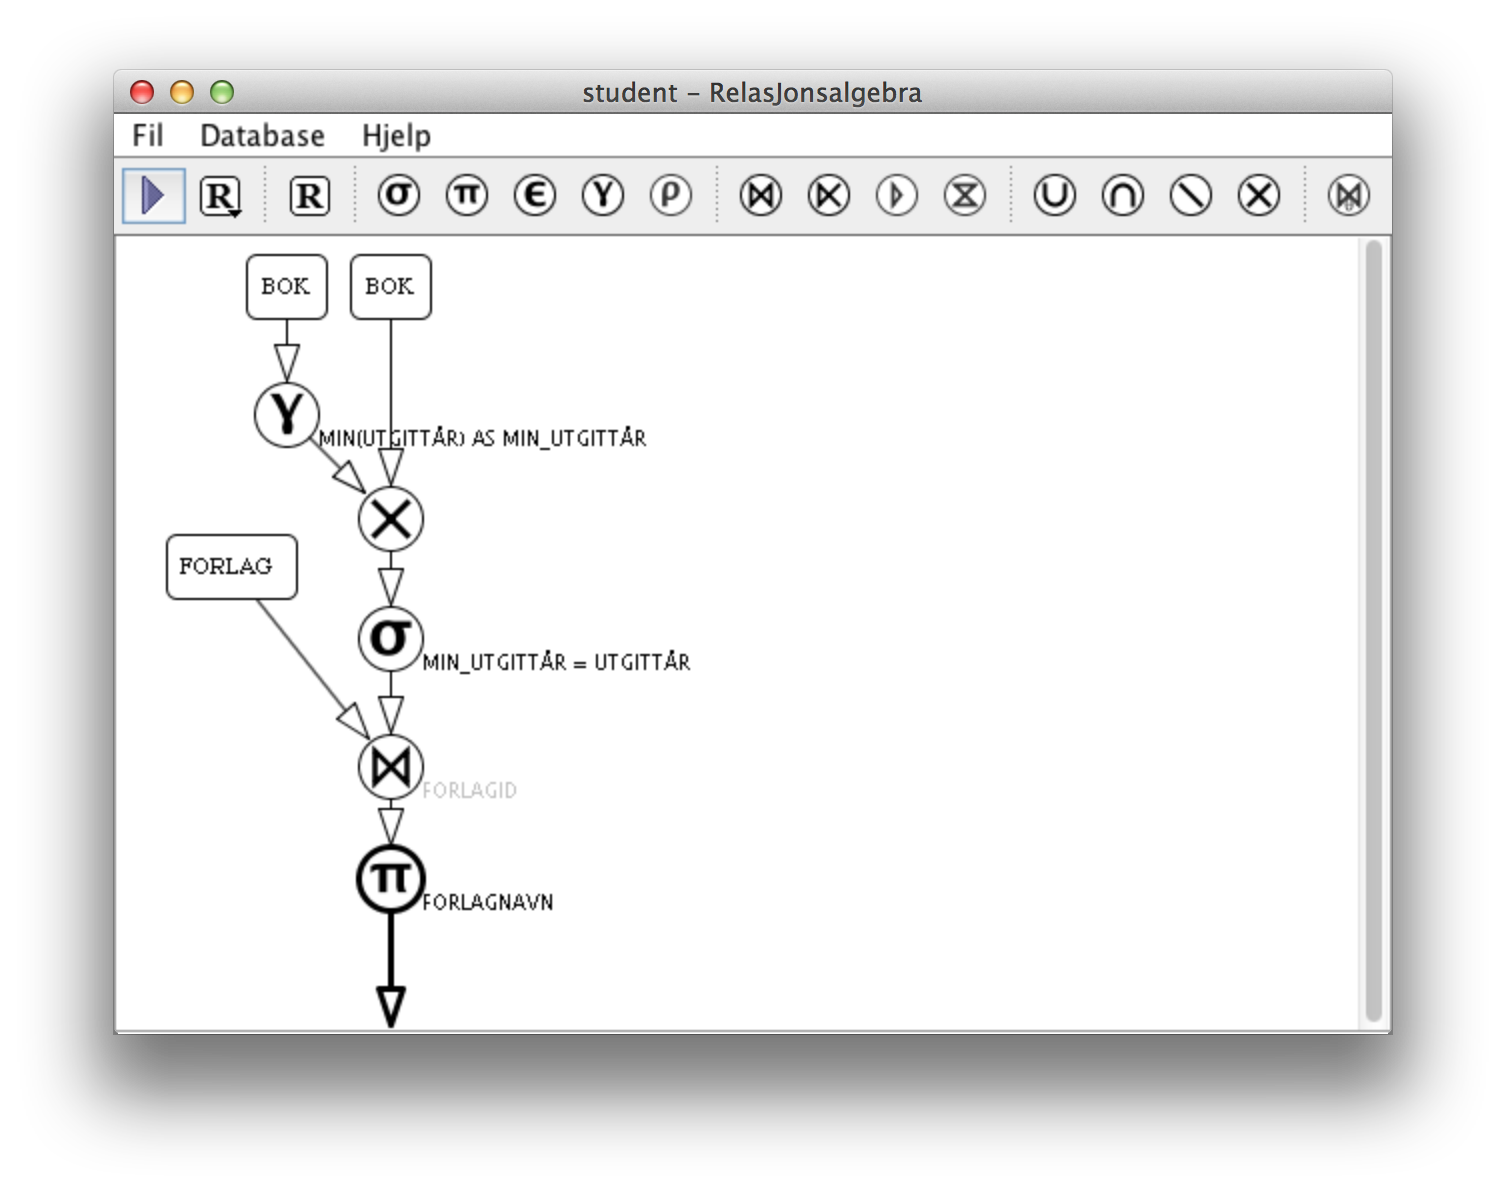
\includegraphics[width=\linewidth]{img/1-10.png}
    \caption{Spørring for oppg. 1.10 \label{img:1.10}}
\end{figure}
\newpage

\subsection{Deloppgave 11}
\begin{figure}[h!]
    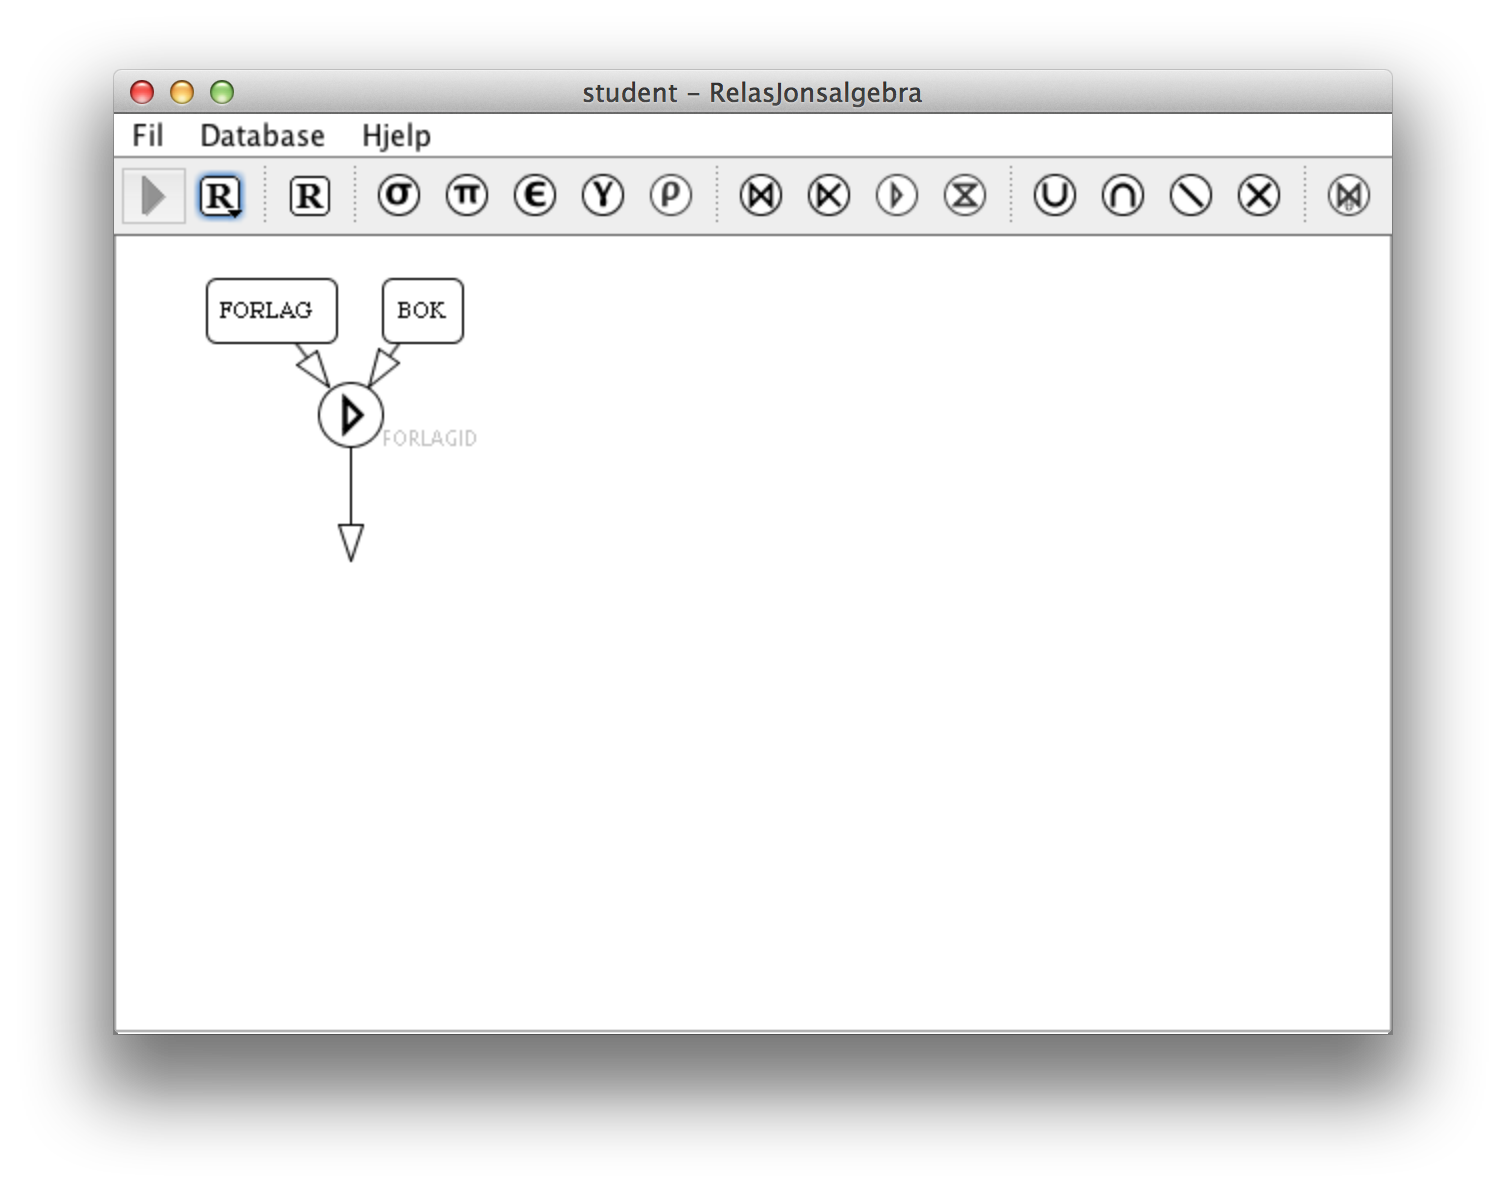
\includegraphics[width=\linewidth]{img/1-11.png}
    \caption{Spørring for oppg. 1.11 \label{img:1.11}}
\end{figure}
\newpage

\section{Oppgave 2}

\lstinputlisting[label=oppg2, caption=Oppgave 2, language=SQL]{opg3.sql}

\section{Oppgave 3}

\subsection{Deloppgave a}

\begin{lstlisting}[language=SQL, label=oppg3a, caption=Oppgave 3a]
mysql> select bok.tittel from bok;
+--------------------------+
| tittel                   |
+--------------------------+
| Taapenes sammensvergelse |
| Rebecca-koden            |
| Gutter er gutter         |
| Microserfs               |
| Generation X             |
| Klosterkronike           |
| Univers uten grenser     |
| Naalen                   |
| Markens Grode            |
| Victoria                 |
| Sult                     |
| Benoni                   |
| Rosa                     |
| Ett skritt etter         |
| Den femte kvinnen        |
| Villspor                 |
| Silkeridderen            |
| Den hvite lovinnen       |
| Hundene i Riga           |
| Bridget Jones dagbok     |
| Sa terapeuten min        |
| Sa mor                   |
| Jubel                    |
| Tatt av kvinnen          |
| NAIV.SUPER.              |
+--------------------------+
25 rows in set (0.00 sec)
\end{lstlisting}


\subsection{Deloppgave b}

\begin{lstlisting}[language=SQL, label=oppg3b, caption=Oppgave 3b]
mysql> select * from forfatter where nasjonalitet = norsk;
+-----+------------+------------+---------+--------+-------------+
| f_id| fornavn    | etternavn  | fodear  | dodar  | nasjonalitet|
+-----+------------+------------+---------+--------+-------------+
|    7| Knut       | Hamsun     |     1859|    1952| Norsk       |
|   11| Lars Saabye| Christensen|     NULL|    NULL| Norsk       |
|   12| Erlend     | Loe        |     NULL|    NULL| Norsk       |
+-----+------------+------------+---------+--------+-------------+
3 rows in set (0.00 sec)
\end{lstlisting}
\newpage

\subsection{Deloppgave c}

\begin{lstlisting}[language=SQL, label=oppg3c, caption=Oppgave 3c]
mysql> select f.forlagnavn, f.telefon
    -> from forlag f 
    -> where adresse = Oslo 
    -> group by f.forlagnavn;
+----------------------+----------+
| forlagnavn           | telefon  |
+----------------------+----------+
| Aschehoug            | 22000000 |
| Cappelen             | 22200000 |
| Gyldendal            | 22220000 |
| Oktober              | 22002200 |
| Tiden                | 22232223 |
| Universitetsforlaget | 23230000 |
+----------------------+----------+
6 rows in set (0.00 sec)
\end{lstlisting}

\subsection{Deloppgave d}

\begin{lstlisting}[language=SQL, label=oppg3d, caption=Oppgave 3d]
mysql> select b.tittel, f.forlagnavn 
    -> from bok b, forlag f
    -> where b.forlagid = f.forlagid;
+--------------------------+---------------+
| tittel                   | forlagnavn    |
+--------------------------+---------------+
| Markens Grode            | Gyldendal     |
| Victoria                 | Gyldendal     |
| Sult                     | Gyldendal     |
| Benoni                   | Gyldendal     |
| Rosa                     | Gyldendal     |
| Ett skritt etter         | Gyldendal     |
| Den femte kvinnen        | Gyldendal     |
| Villspor                 | Gyldendal     |
| Silkeridderen            | Gyldendal     |
| Den hvite lovinnen       | Gyldendal     |
| Hundene i Riga           | Gyldendal     |
| Rebecca-koden            | Cappelen      |
| Klosterkronike           | Cappelen      |
| Univers uten grenser     | Cappelen      |
| Naalen                   | Cappelen      |
| Sa terapeuten min        | Cappelen      |
| Sa mor                   | Cappelen      |
| Jubel                    | Cappelen      |
| Tatt av kvinnen          | Cappelen      |
| NAIV.SUPER.              | Cappelen      |
| Gutter er gutter         | Aschehoug     |
| Bridget Jones dagbok     | Aschehoug     |
| Taapenes sammensvergelse | Tiden         |
| Microserfs               | HarperCollins |
| Generation X             | HarperCollins |
+--------------------------+---------------+
25 rows in set (0.00 sec)
\end{lstlisting}

\subsection{Deloppgave e}

\begin{lstlisting}[language=SQL, label=oppg3e, caption=Oppgave 3e]
mysql> select b.tittel, b.utgittar
    -> from bok b, bokforfatter bf, forfatter f
    -> where bf.bokid = b.bokid
    -> and bf.forfatterid = f.forfatterid
    -> and f.fornavn = Knut
    -> and f.etternavn = Hamsun;
+----------------+-----------+
| tittel         | utgittar  |
+----------------+-----------+
| Markens Grode  |      1917 |
| Victoria       |      1898 |
| Sult           |      1890 |
| Benoni         |      1908 |
| Rosa           |      1908 |
+----------------+-----------+
5 rows in set (0.00 sec)
\end{lstlisting}

\subsection{Deloppgave f}

\begin{lstlisting}[language=SQL, label=oppg3f, caption=Oppgave 3f]
mysql> select f.fornavn, f.etternavn, f.fodear
    -> from forfatter f 
    -> where f.etternavn like H%;
+------------+-----------+----------+
| fornavn    | etternavn | fodear   |
+------------+-----------+----------+
| Stephen W. | Hawking   |     NULL |
| Nick       | Hornby    |     1957 |
| Knut       | Hamsun    |     1859 |
+------------+-----------+----------+
3 rows in set (0.00 sec)
\end{lstlisting}

\subsection{Deloppgave g}

\begin{lstlisting}[language=SQL, label=oppg3g, caption=Oppgave 3g]
mysql> select count(*) from forlag;
+----------+
| count(*) |
+----------+
|        8 |
+----------+
1 row in set (0.00 sec)
\end{lstlisting}
\newpage

\subsection{Deloppgave h}

\begin{lstlisting}[language=SQL, label=oppg3h, caption=Oppgave 3h]
mysql> select b.tittel, f.fornavn, f.etternavn, fl.forlagnavn
    -> from bok b, forfatter f, forlag fl, bokforfatter bf
    -> where bf.bokid = b.bokid
    -> and bf.forfatterid = f.forfatterid
    -> and b.forlagid = fl.forlagid
    -> and f.nasjonalitet = Britisk;
+----------------------+------------+-----------+------------+
| tittel               | fornavn    | etternavn | forlagnavn |
+----------------------+------------+-----------+------------+
| Rebecca-koden        | Ken        | Follet    | Cappelen   |
| Nalen                | Ken        | Follet    | Cappelen   |
| Univers uten grenser | Stephen W. | Hawking   | Cappelen   |
| Gutter er gutter     | Nick       | Hornby    | Aschehoug  |
| Bridget Jones dagbok | Helen      | Fielding  | Aschehoug  |
+----------------------+------------+-----------+------------+
5 rows in set (0.00 sec)
\end{lstlisting}

\subsection{Deloppgave i}

\begin{lstlisting}[language=SQL, label=oppg3i, caption=Oppgave 3i]
mysql> select f.fornavn, f.etternavn, count(*) as antall_boker
    -> from forfatter f, bok b, bokforfatter bf
    -> where b.bokid = bf.bokid
    -> and bf.forfatterid = f.forfatterid
    -> group by f.fornavn, f.etternavn
    -> order by antall_boker desc;
+-------------+-------------+---------------+
| fornavn     | etternavn   | antall_boker  |
+-------------+-------------+---------------+
| Henning     | Mankell     |             6 |
| Knut        | Hamsun      |             5 |
| Ken         | Follet      |             2 |
| Hal         | Sirowitz    |             2 |
| Erlend      | Loe         |             2 |
| Douglas     | Coupland    |             2 |
| John Kenndy | Toole       |             1 |
| Helen       | Fielding    |             1 |
| Stephen W.  | Hawking     |             1 |
| Lars Saabye | Christensen |             1 |
| Jose        | Saramago    |             1 |
| Nick        | Hornby      |             1 |
+-------------+-------------+---------------+
12 rows in set (0.00 sec)
\end{lstlisting}
\newpage

\subsection{Deloppgave j}

\begin{lstlisting}[language=SQL, label=oppg3j, caption=Oppgave 3j]
mysql> select b.tittel, b.utgittar
    -> from bok b
    -> where utgittar = (select min(utgittar) from bok);
+--------+-----------+
| tittel | utgittar  |
+--------+-----------+
| Sult   |      1890 |
+--------+-----------+
1 row in set (0.00 sec)
\end{lstlisting}

\subsection{Deloppgave k}

\begin{lstlisting}[language=SQL, label=oppg3k, caption=Oppgave 3k]
mysql> select f.*, count(*)
    -> from forlag f, bok b
    -> where b.forlagid = f.forlagid
    -> group by f.forlagnavn
    -> having count(*) >= 2;
+----------+---------------+---------+----------+----------+
| forlagid | forlagnavn    | adresse | telefon  | count(*) |
+----------+---------------+---------+----------+----------+
|        5 | Aschehoug     | Oslo    | 22000000 |        2 |
|        3 | Cappelen      | Oslo    | 22200000 |        9 |
|        2 | Gyldendal     | Oslo    | 22220000 |       11 |
|        8 | HarperCollins | USA     | NULL     |        2 |
+----------+---------------+---------+----------+----------+
4 rows in set (0.00 sec)
\end{lstlisting}

\subsection{Deloppgave l}

\begin{lstlisting}[language=SQL, label=oppg3l, caption=Oppgave 3l]
mysql> select *
    -> from forlag
    -> where forlagid not in (select b.forlagid from bok b)
    -> group by forlagnavn
    -> order by forlagid;
+----------+----------------------+-----------+----------+
| forlagid | forlagnavn           | adresse   | telefon  |
+----------+----------------------+-----------+----------+
|        1 | Tapir                | Trondheim | 73590000 |
|        4 | Universitetsforlaget | Oslo      | 23230000 |
|        6 | Oktober              | Oslo      | 22002200 |
+----------+----------------------+-----------+----------+
3 rows in set (0.00 sec)
\end{lstlisting}

\section{Oppgave 4}

\subsection{Deloppgave a}


Hensikten med views er å kunne samle alle eller deler av atributtene i en tabell i en ny samling av atributter som forklarer noe annet en den/de opprinnelige tabellen(e) forklarte uten å skape redundans.


Det kan oppstå problemer rundt oppdatering eller innsetting i views ettersom det i mange tilfeller ikke er helt klart hvordan disse operasjonene skal gjenspeiles i de originale tabellene. Generelt sett er det frarådd å oppdatere gjennom views.


\subsection{Deloppgave b}

\begin{lstlisting}[language=SQL, label=oppg4b, caption=Oppgave 4b]
create view project_overview(p_name, d_name, e_count, h_count)
as select p.pname, d.dname, count(*), sum(w.hours)
from project p, department d, works_on w
where p.dno = d.dnumber
and p.pnumber = w.pno
group by p.pname;
\end{lstlisting}

\subsection{Deloppgave c}

\subsubsection{Deloppgave 1}

\begin{lstlisting}[language=SQL, label=oppg4c1, caption=Oppgave 4c1]
select DNO, count(*), sum(SALARAY), avg(SALARY)
from EMPLOYEE
group by DNO;
\end{lstlisting}

\subsubsection{Deloppgave 2}

\begin{lstlisting}[language=SQL, label=oppg4c2, caption=Oppgave 4c2]
select DNO, count(*)
from EMPLOYEE
having sum(SALARY) > 10000
group by DNO;
\end{lstlisting}

\subsubsection{Deloppgave 3 og 4}

Disse er ikke lovlige oppdateringer ettersom viewen inneholder aggregater.

\newpage
\section{Oppgave 5}

\subsection{Deloppgave a}

\begin{lstlisting}[language=SQL, label=oppg5a, caption=Oppgave 5a]
select * 
from Supplier
where status > 15;
\end{lstlisting}

\subsection{Deloppgave b}

\begin{lstlisting}[language=SQL, label=oppg5b, caption=Oppgave 5b]
select s.sname, s.city 
from Supplier s, Part p, SuppliesPart sp
where s.sno = sp.sno 
and sp.pno = p.pno 
and p.pname = Screw;
\end{lstlisting}

\subsection{Deloppgave c}

\begin{lstlisting}[language=SQL, label=oppg5c, caption=Oppgave 5c]
select p.pno, p.pname 
from Part p 
where p.pno in (select pno from SuppliesPart group by pno having count(*) > 1);
\end{lstlisting}

\subsection{Deloppgave d}

\begin{lstlisting}[language=SQL, label=oppg5d, caption=Oppgave 5d]
select count(*) as total 
from Supplier;
\end{lstlisting}

\subsection{Deloppgave e}

\begin{lstlisting}[language=SQL, label=oppg5e, caption=Oppgave 5e]
select s.city 
from Supplier s, SuppliesPart sp, Part p 
where s.sno = sp.sno 
and sp.pno = p.pno 
and p.weight > 10 
group by s.city;
\end{lstlisting}

\newpage
\subsection{Deloppgave f}

\begin{lstlisting}[language=SQL, label=oppg5f, caption=Oppgave 5f]
select distinct s.sname
from Supplier s
where s.sno not in (
    select s.sno
    from Supplier s, SuppliesPart sp, Part p
    where s.sno = sp.sno
    and sp.pno = p.pno
    and p.pname = Screw)
order by s.sname;
\end{lstlisting}
\end{document}
